\documentclass[12pt]{article}

\usepackage[margin=1.4in]{geometry}
\usepackage{amsmath}
\usepackage{graphicx}
\graphicspath{{./figures/}}

\begin{document}
\begin{titlepage}

\begin{center}
\begin{huge}
Audio Compression\\
\end{huge}
14-bit to 8-bit\\
\vspace{1.5cm}
\textbf{Duncan MacDonald}\\
duncmac.16@gmail.com\\
V00842740\\
\vfill
SENG 440 - Embedded Systems\\
University Of Victoria\\
Department of Engineering\\
\vspace{1.5cm}
\today
\end{center}
\end{titlepage}
\newpage
\tableofcontents
\listoffigures
\newpage
\section{Introduction}
\indent 
Recording audio and storing it digitally, in its fullest form is a very costly process; the same goes for transmitting it. For that reason, audio compression came to be. There are two type of audio compression methods, lossless and lossy, this report will be going over the latter, specifically $\mu$-law and $A$-law. Even though $\mu$-law does loss some data in compression, it's usage is still justified in telecommunication as it makes data transfer a lot faster with little noticeable to the human ear[1].\\

$\mu$-law takes in a 14-bit sample of the recorded signal and creates a logarithmic approximation of the signal recording the position of the most significant bits and the step of the preceding bits. This project in particular is an implementation of $\mu$-law used on to compress a audio file and uses the inverse to expand it back to a usable file. After the initial implementation was create, multiple different optimization techniques were preformed to the algorithm to take the highest traffic parts and reduce the instructions needed to complete them. After the software optimizations were completed, hypothetical hardware assisted were added to the algorithm to increase the speed of the algorithm even further.\\

The resulting algorithm would be the base to a highly optimized embedded system could be further implemented with hardware to be used in a production setting. The following report highlights the background knowledge the algorithm it is based on, the optimization techniques used in the software and performance analysis on all stages of the design.\\
 
\section{Background}

The basis of why the data lost in compression is justifiable is the characteristics of human speech[1]. Most of the things people say vocally are of a much higher amplitude than things such as background noise or sounds of friction of things around the recording device[1]. This is why compressing large signals of vocal sounds is affordable, since the lower amplitude signals of non-vocal sounds aren't really relevant to the transfer of human voice. \\

The way that \texttt{.wav} files are recorded is in uniformly spaced quantized values of a signal, with lower levels of noise recorded with fewer bits and larger levels of noise recorded with more bits. This is referred to as uniform pulse code modulation[1]. The idea behind such codec as $\mu$-law and $A$-law is to take a logarithmic representation of the uniformly spaced signals so that an 8-bit code can represent the potentially larger signal. \\

\begin{align}
y = sgn(x)\frac{ln(1+\mu|x|)}{ln(1+ \mu)}\\
y = \begin{cases}
sgn(x)\frac{A|x|}{1+ln A} \\
sgn(x)\frac{1+ln(A|x|)}{1 + ln A}\\
\end{cases}
\end{align}

$\mu$-law, represented by equation 1 is the function that is to be implemented in software, where $\mu$ is a parameter that can range from 0 (no compression) to 255 (maximum compression)[1]. To implement this in software, the software is going to use a piecewise logarithmic approximation of this equation to compress a signal. Inversely, the software is going to use exponentials to expand the compressed codec into something useful again. \\

\section{Design}

\subsection{Modelling}

To create a basis of how the program was going to work, the first needed to be done was to model the program with a UML diagram. Using this would create a generic overview of how the program was going to flow and what components need to created in high-level terms. There was some deviation from this diagram in the first iteration of creating the code for the sake of readability, but the algorithm remained somewhat the same going from UML to C. 

\begin{figure}[!h]
	\centering
	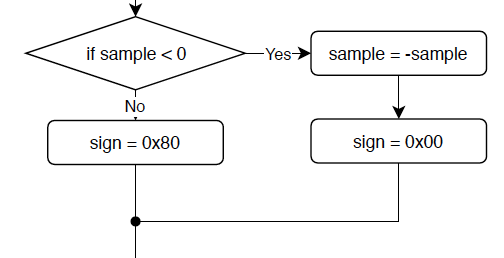
\includegraphics[scale=1]{mag_uml.png}
	\caption{\label{fig:mag_uml}UML diagram of procedure that takes place when finding magnitude.}
\end{figure}

The first thing that is done after the initialization of the variables, is the magnitude of the sample is found. When this happens, the flip of the last bit is store and the magnitude is kept for the rest of the processing. \\

\begin{figure}[!h]
	\centering
	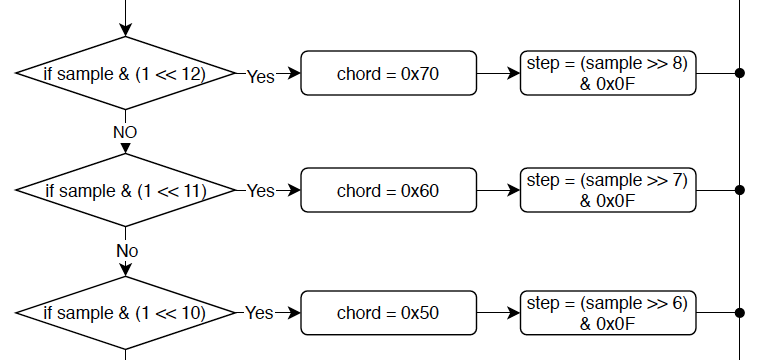
\includegraphics[scale=1]{step_uml.png}
	\caption{UML diagram of procedure that takes place when finding the piecewise log of the sample.}
\end{figure}

After the magnitude is found, the piecewise log is found and stored and then the 4 bits after wards are stored as the step of the value. Out of the scope of the figure is all of these components together in a loop, storing the results in an area. This deviates from what was actually code for the arm controller, as there was only a test suite set up for a select few values.

\subsection{Design Methodology}

For a design methodology, I used a low cost version of test driven development. To produce some samples I made a 16-bit integer as a pseudo-sample and compressed it into a code word and expanded it again. In the end of the first iteration, some of the samples produced by the testing did not expand back in the same format, but it was expected since the samples produced were not in the format of a 14-bit quantized value. The rest of the values expanded in a similar fashion, only keeping the five or six most significant figures and dropping the rest. The samples produced were dispersed throughout a range of different chords and steps so that all aspects were tested. I used a for loop as seen in figure 1 that takes the initial sample and shifts it over one space, clearing the most significant bit and compresses and decompresses sample and displays the results. This was then repeat with a different step to ensure that the steps were correctly being compressed. As I mentions before this was a low cost testing method, so no actual testing software was used. Using a form of test driven development was very helpful though, as bugs that occurred were quickly seen and corrected.\\

\begin{figure}[!h]
        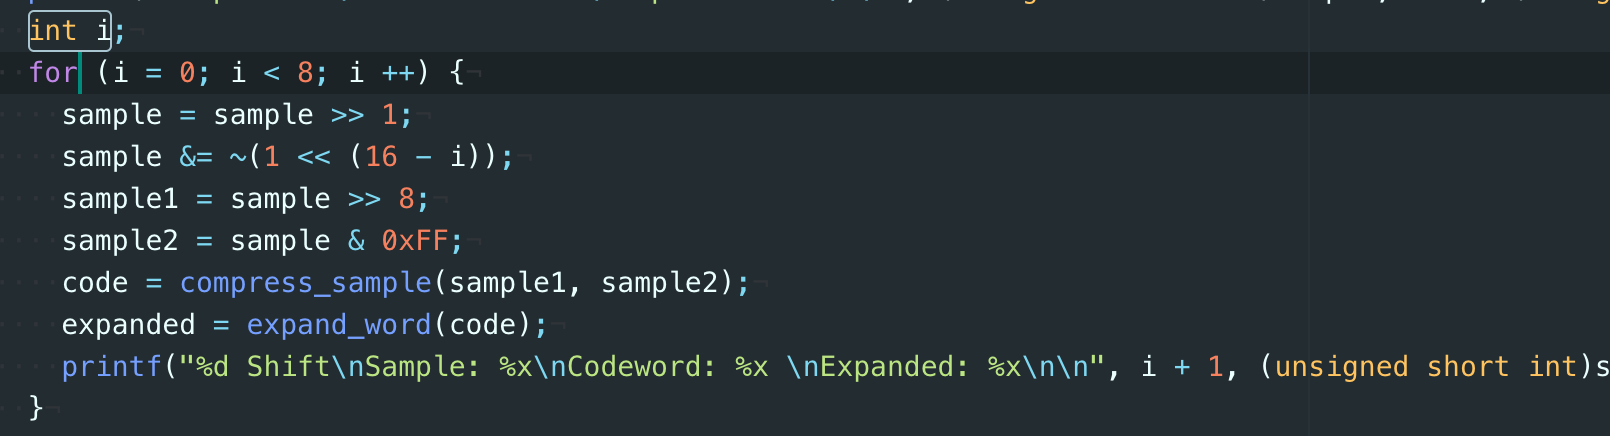
\includegraphics[width=\textwidth]
        {testingLoop.png}
        \caption{\label{fig:test_loop} Testing for loop to produce samples to compress}
\end{figure}


\subsection{Original Design}

In the actual implementation of the algorithm, the program would take in a file and write the data into a struct with a place for a header, data and the size of the data. The first thing that was done was removing the head from the original file and placing it in the compressed file. After this was done the data, in the form of 8 bit character data type were compressed, this was done by first getting the sign of the character, the magnitude of the character, the chord and step. After the values were found, they were connected together into one code word and written into the \texttt{Compressed} struct. The header and the compressed data was then written into a file.\\

The sign, step and chord were found through functions calls in the first iteration for the sake of convenience and readability. This was done knowing that it would later have to be optimized, but I thought it would be better to get the algorithm complete and readable before I started optimizing the code. There were multiple different things I did to get more out of readability and harm on speed performance. An example of this can be seen in figure \ref{fig:test_loop}, where I used a for loop to cycle through cases to find the leading bit.\\

\begin{figure}[!h]
		\centering
        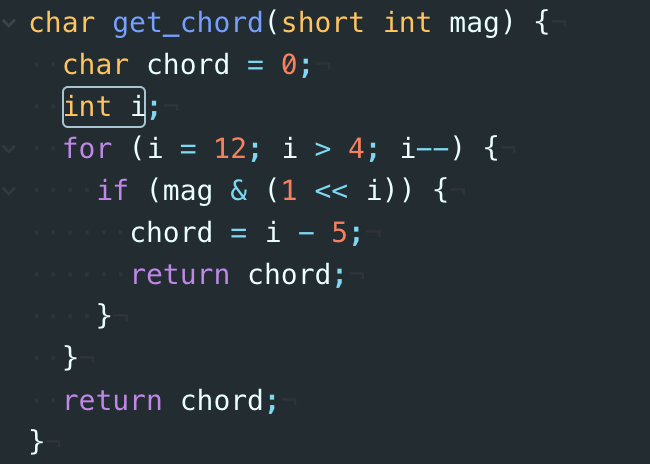
\includegraphics[width=10cm ]
        {get_chord_for_loop.png}
        \caption{\label{fig:chord_loop} For loop used to find the leading one bit.}
\end{figure}

\subsection{Optimizations}

To optimized the code, the parts of the code looked at were the parts that were called the most. All of the parts of code having to do with the compression and expansion could be improved by quite a bit. The first thing that was done to optimize the code is to remove the for loop shown in figure \ref{fig:chord_loop}. Using a for loop creates a significant amount of branching added instructions to increment the loop. There is also a lot of extra math that could be avoided. So the result of optimization produced a long string of if else statements. \\

To optimize the compression further, all of the functions in the code to find the different sections of the code words were put into the same function. Doing this takes away the overhead of stack pushing and popping. After all of the function were brought together, the values that were previously returned using math were hard coded save on operations. The bit values were written in the way that they would be in the code word (ex. finding a chord of \texttt{0x4} would result in \texttt{0x40}). This helps save operations on shifting bits over when combining the values of step, chord and sign together. \\

Another aspect of the code that was changed to reduce time is using the \texttt{register} key for the  \texttt{sample} variable. This being a highly modified value, it is important to remove the overhead of having to look in memory for this variable.\\

\subsection{Hardware Design}

To design hardware for the system, the bottle neck of the system had to be identified. This was definitely the actual compression or decompression part of the algorithm as it would be called for each sample in the file or the stream going into or out of the system. In the program that compresses a whole \texttt{.wav} file. The algorithm first removes the header of the file, because the information in that cannot be lossy, then it goes through all of the samples in the file and compresses them into code words. Because the head is under 100 bytes of information and the body contains a significant more than that, the bottle neck of the system would benefit greatly if there the samples were compressed through hardware. \\

\subsubsection*{VHDL}

To model the compression of the algorithm, the algorithm was redesigned in VHDL, a hardware description language. This was useful to use as it simulated the logic of designing a circuit without having to actually design it. In the hardware model, there would be an input for the mode of either compression or decompression, and an input of either the codeword or sample sample. The output would be either the compressed sample or decompressed codeword respective to the mode that the hardware was in. \\

\begin{figure}[!h]
		\centering
        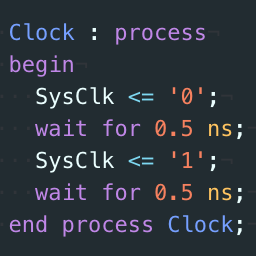
\includegraphics[width=6.5cm ]
        {clock_comp.png}
        \caption{\label{fig:clock_comp} Clock component used in VHDL simulation.}
\end{figure}


To implement this in VHDL, there needed to be an architecture to have a test bench and a flow throughout the system. The main component of the system is the \texttt{Clock} process as seen in figure \ref{fig:clock_comp}. This component is responsible for creating all of the values and generating the signals for the compression and decompression methods. The \texttt{SysClk} signal is a value of one or zero that is updated every nanosecond. On every rising edge of the \texttt{SysClk} the \texttt{input1} signal is incremented by one and sent in the ulaw. The \texttt{input1} is used by both the compression and decompression processes for the sake of being able to see the samples going into the system and the samples going out of the system. The other part of the simulation is the simulation process; since this process is running concurrently with the rest of the program, it will be able to stop the simulation once it has reach a time when all of the values have entered into the system.\\

Together, the clock signal drives the incrementation of the inputs going into the compression and decompression until the simulation process finishes. In the actual algorithm, it works similarly to the C implementation, for the sake of having a work bench, all of the values used by the compression and decompression processes are outputted. Since these processes run concurrently, both the code word going out of the compression and the code word going into the decompression process were recorded because the decompression method would happen faster than the compression method and not update the signal until after the compression process was done. This phenomenon can be seen in figure \ref{fig:concur}.\\

\begin{figure}[!h]
		\centering
        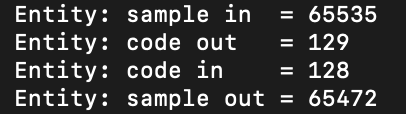
\includegraphics[width=8cm]
        {concur.png}
        \caption{\label{fig:concur} Concurrency in action in during simulation.}
\end{figure}

The mode component was added to the entity, but not actually implemented, since it would be trivial to add, make it a lot harder to test. This was also true for the output in the \texttt{ulaw} entity. The resulting assembly operation would be \texttt{ulaw Rs Rm Rt} as suggested by Dr.Sima's slides, where Rs is the source operand, Rm would be mode and Rt is the target operand where the results would be stored[1]. Since ARM is a 32-bit processor, it would all 32-bit words, but not all of the bits would be used. A VHDL representation of the operator can be seen in figure \ref{fig:ulaw_entity}.\\



\begin{figure}[!h]
		\centering
        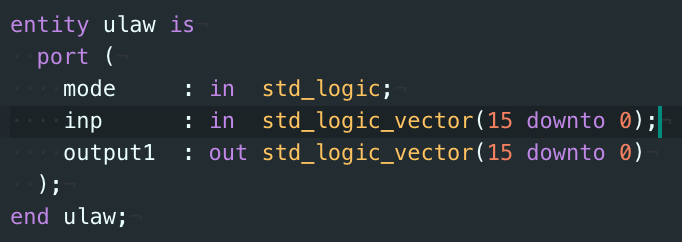
\includegraphics[width=8cm]
        {ulaw_entity.png}
        \caption{\label{fig:ulaw_entity} Concurrency in action in during simulation.}
\end{figure}

\section{Performance}



\section{Conclusion}

Sending audio signals in there fullest uniformly pulsated state is very costly in the amount of data needed to be sent.The characteristics of the human voice and auditory system as such that people do not need to hear lower amplitude sound. This gives reason to use such codecs as $A$-law and $\mu$-law to compress these signals into something that is both smaller than the original signal and recognizable to the human ear even if there is some data lost in compression. 

The piecewise logarithm method, implementable in software, is a good way to approximate $\mu$-law to preform a lossy compression of audio samples. The algorithm was first implemented as a UML diagram to complete the requirements of the system and then converted into C code. After the C code was optimized to preform the same task in fewer instructions and less looking in memory. The assembly code was then generate through the \texttt{gcc} and more unnecessary instructions were taken out. After this was done, a simulation of the hardware that would replace this compression method was designed and tested. Finally, the hypothetical instruction described by the simulation replaced the $\mu$-law compression and expansion methods and the instruction count with the estimated latency of new instruction was used to analyse the performance of system with no optimizations, the system with optimizations, and the system with simulated hardware involved.\\

Audio compression, software optimization and hardware design are what make such systems as telecommunications possible. These techniques and practices are permeated throughout the design world and are an import to having high performing systems.\\
   

\newpage
\section{Bibliography}
[1] M.Sima, ``SENG 440 Lesson 101 Project ‘Audio Compression’" $[$Online Document$]$\\
http:\/\/www.ece.uvic.ca\/~msima\/TEACHING\/COURSES\/SENG\_440\/
PROTECTED\/SLIDES\\\/SENG\_440\_slides\_Lesson\_project\_101.pdf\\
$[$ Last accessed July 31 2019 $]$
\end{document}